
\chapter{Arquitetura}
\label{sec:arquitetura}

A arquitetura é uma etapa fundamental em todos os projetos porque é aqui que se define a estrutura e comportamento do sistema na sua globalidade e nas diferentes componentes.

Neste capítulo está exposta a arquitetura do 10.quest que servirá de \textit{guideline} para a implementação do projeto. Serão apresentadas diferentes perspetivas para analisar os diferentes aspetos do sistema. É de notar que as componentes a desenvolver pela restante equipa de desenvolvimento não serão analisadas e apenas serão apresentadas de forma superficial para fazer a ligação às componentes a desenvolver no âmbito do estágio curricular.
Este capítulo é também uma exposição das decisões arquiteturais efetuadas no primeiro semestre, respeitando as restrições técnicas e de negócios.

Por fim apresenta-se uma análise dos riscos envolvidos no desenvolvimento do projeto, o seu impacto e probabilidade de ocorrência e o respetivo plano de mitigação.




\section{Análise da Arquitetura}
\label{analisearq}

Na análise da arquitetura serão apresentadas as restrições do projeto, que têm um impacto direto nas decisões de arquitetura, nas diferentes perspetivas de arquitetura e nas tecnologias utilizadas.

\subsection{Restrições Técnicas}
As restrições técnicas são decisões técnicas arquiteturais que devem ser satisfeitas. O sistema a desenvolver deve respeitar as seguintes restrições:

\textbf{Identificador: RT01}
\newline
\textbf{Título:} Arquitetura REST
\newline
\textbf{Descrição:} A comunicação entre a plataforma a desenvolver e o TCG deve seguir uma arquitetura REST.

\textbf{Identificador: RT02}
\newline
\textbf{Título:} Base de Dados
\newline
\textbf{Descrição:} Os dados utilizados pela aplicação devem ser guardados numa base de dados, visto tratar-se de um grande volume de dados que tem de permanecer organizado. Relativamente aos dados do TCG foi imposto que apenas uma pequena porção dos dados sejam duplicados (i. e. em ambas as bases de dados), e toda a informação seja acedida através de pedidos \acrshort{https}/\acrshort{rest}. PostgreSQL\cite{sql} é a base de dados relacional utilizada pela empresa e portanto será também utilizada no desenvolvimento deste projeto.

\textbf{Identificador: RT03}
\newline
\textbf{Título:} Framework Django\cite{django}
\newline
\textbf{Descrição:} A Framework Django é a tecnologia utilizada pela empresa para desenvolver aplicações \textit{web} e \textit{\acrshort{saas}}. O uso desta tecnologia foi imposta pelo \textit{Product Owner}.

\textbf{Identificador: RT04}
\newline
\textbf{Título:} Plataforma Web
\newline
\textbf{Descrição:} Todas as funcionalidades do sistema devem estar disponíveis através da plataforma web.

\subsection{Restrições de Negócio}
Nesta secção estão descritas as restrições de negócio, que podem ser entendidas como barreiras pelas quais a organização deve lutar para executar a sua estratégia. Estas restrições, que apresento em seguida foram impostas pelo \textit{Product Owner} e devem ser satisfeitas na arquitetura do sistema:

\textbf{Identificador: RN01}
\newline
\textbf{Título:} Programa de Desenvolvimento
\newline
\textbf{Descrição:} O produto deve estar concluído e validado até dia 30 de Outubro.



\subsection{\acrfull{mvc}}

A estrutura de um projeto Django é muitas vezes descrito como um projeto \acrshort{mvc}. Como podemos ver na Figura \ref{fig:arq-mvc}, o modelo \acrshort{mvc} é uma arquitetura de software que separa a aplicação em três componentes lógicos principais. Por outras palavras este modelo separa a apresentação dos dados, da lógica que trata das \textit{interfaces} do utilizador, facilitando a programação das diferentes funcionalidades, \textit{debugging} e os testes das mesmas.

\begin{figure}[ht!]
	\begin{center}
		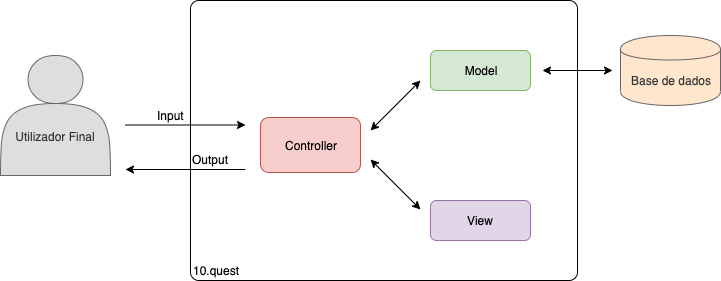
\includegraphics[width=1\textwidth]{img/arq/diagrama-MVC}
		\caption{Estrutura do Sistema}
		\label{fig:arq-mvc}
	\end{center}
\end{figure}

O componente \textbf{Model} controla a organização e armazenamento dos dados. Este módulo representa os dados que são transferidos entre os componentes Controller e View mas não representa nenhuma lógica no que diz respeito ao que é representado na camada de apresentação.

O componente \textbf{View} pode ser considerada a camada de apresentação. Este componente contém todas os ingredientes que constituem as interfaces do utilizador e controla a forma como a informação lhe é apresentada. Este modelo sabe como aceder ao modelo de dados que é apresentado ao utilizador contudo não sabe como o manipular nem o que significa.

Por último temos o componente \textbf{Controller}.  Este componente atua entre os modelos View e Model reagindo a eventos na View e respondendo a estes pedidos manipulando os dados utilizando o componente Model e interagindo com o componente View para renderizar o \textit{output}.


\subsection{Modelo C4}

Nesta secção encontra-se representada e descrita toda a arquitetura da plataforma 10.quest,  influenciada pelos objetivos de negócio, \textit{stakeholders}, requisitos e restrições técnica e de negócio, apresentados anteriormente.

Foram utilizados três diagramas para representar a arquitetura do sistema, utilizando o \textbf{modelo C4}\cite{c4}: diagrama de contexto, diagrama de contentores e o diagrama de componentes.

Os diferentes diagramas representam diferentes perspetivas e níveis de abstração e foram feitos com o intuito de facilitar a compreensão da arquitetura permitindo à equipa de desenvolvimento visualizar os diferentes níveis de granularidade. 

O diagrama de contexto mostra a relação entre o sistema que vai ser desenvolvido e outros agentes como, por exemplo, utilizadores e sistemas externos.  Este é o diagrama com maior nível de abstração e é bom para sublinhar as dependências externas que a equipa de desenvolvimento tem que integrar no sistema. 

O diagrama de contentores apresenta um maior detalhe (i. e. relativamente ao diagrama de contexto) e mostra os diferentes contentores que constituem o sistema (e. g. bases de dados, aplicações, microserviços etc...). Neste diagrama são também definidas algumas decisões arquiteturais. 

Por último temos o diagrama de componentes que aproxima um contentor individualmente e mostra todos os componentes que constituem esse contentor. Desta forma conseguimos perceber as principais funcionalidades do sistema. 


\subsubsection{Diagrama de Contexto}

Como foi referido no Capítulo \ref{sec:introducao} o 10.quest é uma plataforma de inbound marketing que consiste num \textit{backoffice} para a criação de campanhas. Estas podem ser questionários de personalidade, concursos e/ou formações, sendo que a última é criada com auxílio do \acrshort{tcg}.

Como podemos ver na Figura \ref{fig:arq-contexto} o 10.quest interage com seis sistemas externos. O SendGrid\cite{sg} é um \acrshort{saas}, na \textit{cloud}, que fornece um serviço de entrega de emails. Este serviço permite enviar emails através de APIs flexíveis garantindo uma disponibilidade  de 99.999\% \cite{sguptime}. 
O TCG, tal como foi referido no Capítulo \ref{sec:estado-arte}, é uma plataforma de criação de formações que tem como principal objetivo, transmitir conhecimento através de uma técnica de aprendizagem baseada em tentativa e erro. Algumas das funcionalidades do \acrshort{tcg} serão utilizadas pelo 10.quest.
Para partilhar campanhas, o 10.quest irá utilizar as APIs do Facebook, LinkedIn e Twitter.


\newpage

\begin{figure}[ht!]
	\begin{center}
		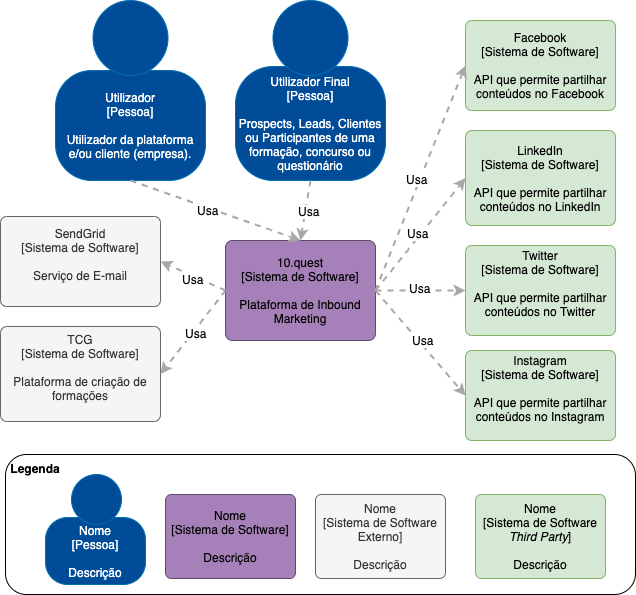
\includegraphics[width=0.9\textwidth]{img/arq/diagrama-contexto}
		\caption{Diagrama de Contexto}
		\label{fig:arq-contexto}
	\end{center}
\end{figure}

\subsubsection{Diagrama de Contentores}

Na Figura \ref{fig:arq-contentores} está representado o diagrama de contentores, onde se pode observar com mais detalhe a constituição do sistema de software.

Os utilizadores podem ser de dois tipos: o utilizador do backoffice (i. e. utilizador da plataforma) que tem acesso a todas as funcionalidades da plataforma e o utilizador final que tem acesso a uma página web para participar nas campanhas.

A aplicação web efetua os pedidos dos utilizadores, através de pedidos \acrshort{https}/\acrshort{rest} à API. A aplicação web será a camada de apresentação da API e ambos serão desenvolvidos em Django. A API será o contentor responsável por tratar de todos os pedidos efetuados pelos utilizadores do \textit{backoffice}. Para este efeito a API implementa um conjunto de funcionalidades, representadas na Figura \ref{fig:arq-componentes1}, que manipulam um conjunto de dados armazenados numa base de dados relacional PostgreSQL, para conseguir as informações necessárias.
\newpage

\begin{figure}[ht!]
	\begin{center}
		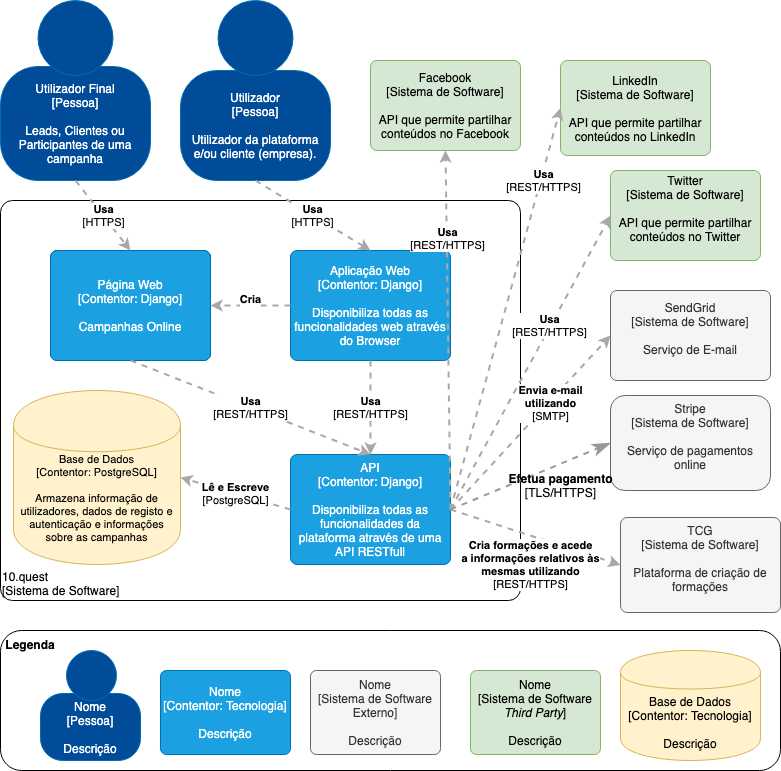
\includegraphics[width=0.9\textwidth]{img/arq/diagrama-contentores}
		\caption{Diagrama de Contentores}
		\label{fig:arq-contentores}
	\end{center}
\end{figure}

\subsubsection{Diagrama de Componentes}

Na Figura \ref{fig:arq-componentes} é apresentado o diagrama de componentes e na Figura \ref{fig:arq-componentes1} são apresentados os componentes da API. 

A autenticação é necessária para que os pedidos sejam aceites e mapeados pela API. Para isto a componente "Autenticação", permite ao utilizador efetuar a sua autenticação e verifica a autenticidade do mesmo, em cada pedido, através de tokens. Desta forma, caso o utilizador esteja autenticado os seus pedidos \acrshort{https}/\acrshort{rest} avançam para a componente API , que inclui todas as componente (i. e. funcionalidades) que dão resposta aos requisitos funcionais definidos para o projeto.

A componente "Dados" permite às restantes componentes interagir com a base de dados, tanto para ler, como para escrever.

\newpage

\begin{figure}[ht!]
	\begin{center}
		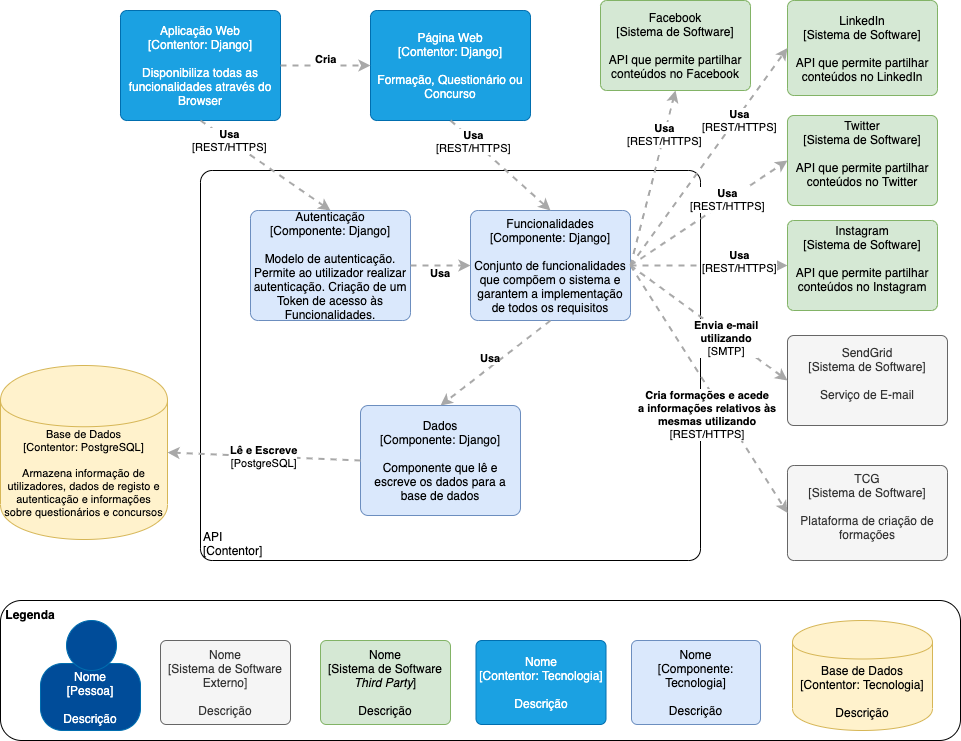
\includegraphics[width=0.83\textwidth]{img/arq/diagrama-componentes}
		\caption{Diagrama de Componentes}
		\label{fig:arq-componentes}
	\end{center}
\end{figure}

\begin{figure}[ht!]
	\begin{center}
		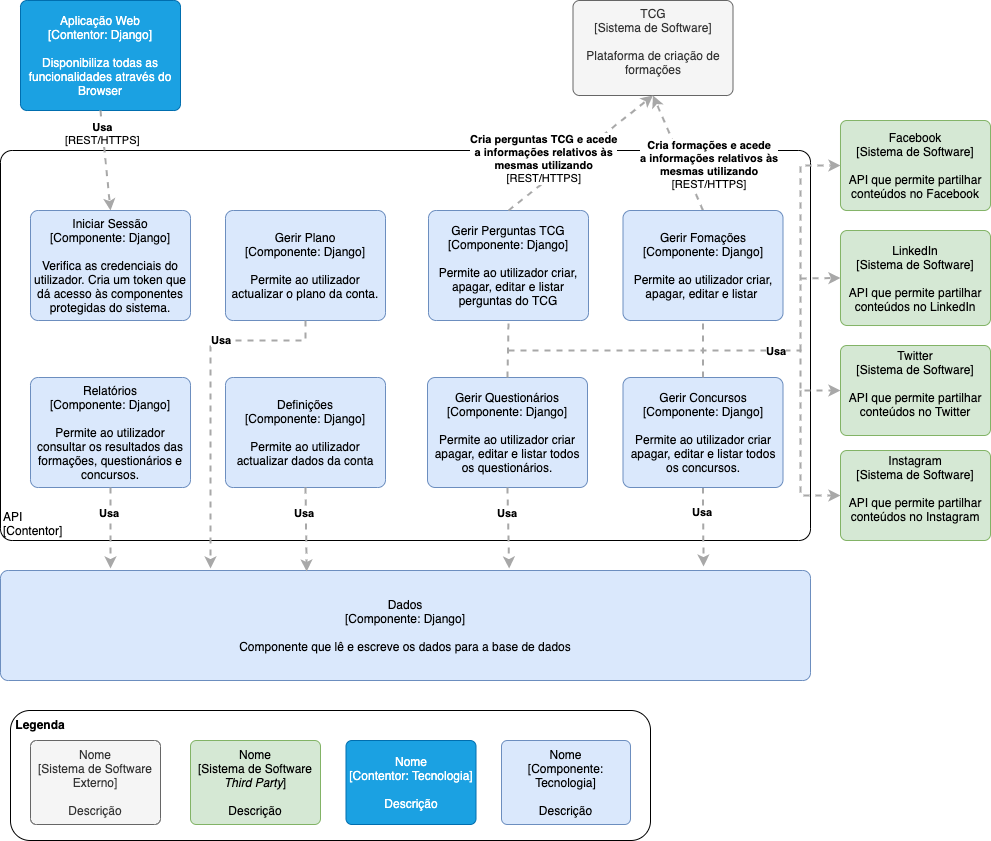
\includegraphics[width=0.83\textwidth]{img/arq/diagrama-componentes1}
		\caption{Diagrama Componentes da componente Funcionalidades}
		\label{fig:arq-componentes1}
	\end{center}
\end{figure}

\newpage


\subsection{Diagrama Entidade Relacionamento}

Nesta secção é apresentado o diagrama conceitual que representa a base de dados do projeto desenvolvido. De seguida é dada uma breve descrição de todas as classes presentes na Figura \ref{fig:arq-er}. 

\begin{figure}[ht!]
	\begin{center}
		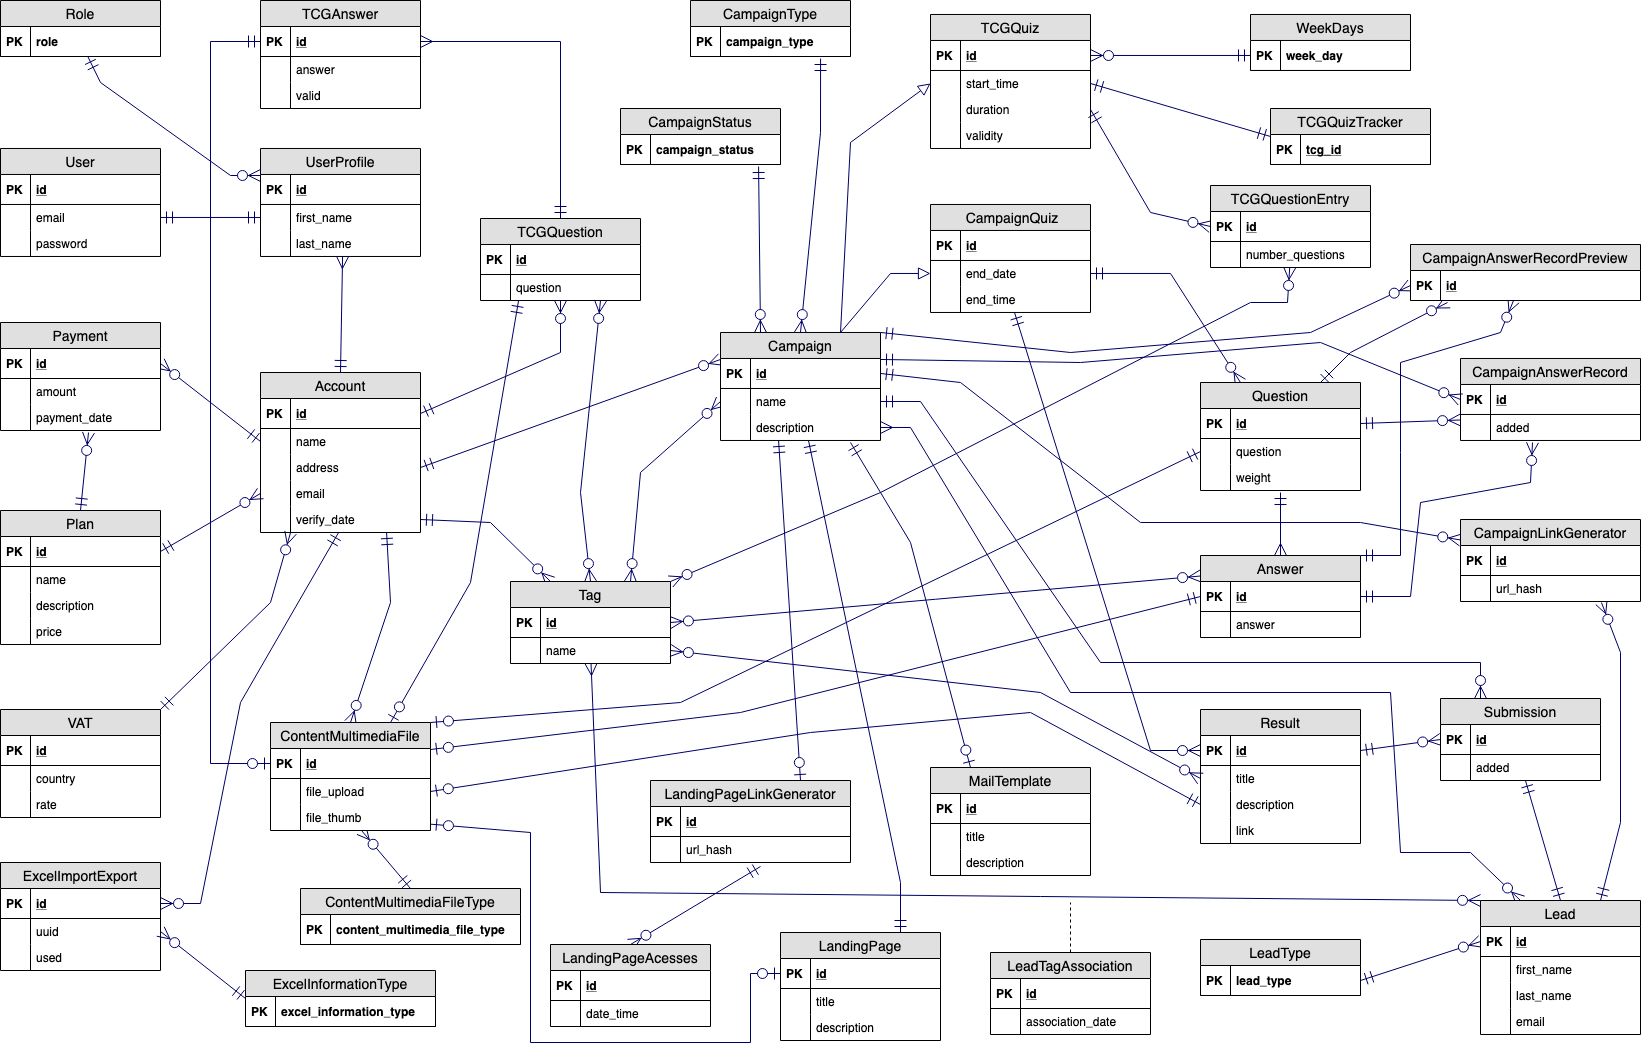
\includegraphics[width=0.87\textwidth]{img/arq/er}
		\caption{Diagrama Entidade Relacionamento - Modelo Conceitual}
		\label{fig:arq-er}
	\end{center}
\end{figure}

Com o diagrama representado na Figura \ref{fig:arq-er} consegue-se perceber quais são as entidades e como se relacionam entre si, dentro do sistema.

\begin{itemize}
	\item[--] \textbf{ContentMultimediaFile}: Esta entidade representa o conteúdo multimédia carregado pelos utilizadores na plataforma. Está diretamente relacionado com:
	\subitem \underline{Account}: Um conteúdo multimédia está associado a uma conta de empresa.
	\subitem \underline{ContentMultimediaFileType}: Um conteúdo multimédia por ser uma imagem ou um vídeo.
	\item[--] \textbf{VAT}: VAT (\textit{Value Added Tax}) representa o imposto correspondente a cada país.
	\item[--] \textbf{Tag}: Esta entidade representa uma tag. Estas tags são associadas a outras entidades para traçar características da mesma:
	\subitem \underline{Account}: Uma tag está associada a uma conta de empresa.
	\subitem \underline{Campaign}: Uma campanha pode ter múltiplas tags que serão associadas mais tarde aos participantes da mesma.
	\subitem \underline{Result}: Um resultado pode ter múltiplas tags que serão associadas aos participantes a quem saia o mesmo.
	\subitem \underline{TCGQuestion}: Uma pergunta de uma formação pode ter múltiplas tags associadas.
	\subitem \underline{TCGQuestionEntry}: Uma entrada de perguntas de formação, pode ter múltiplas tags que representam as perguntas que têm essas mesmas tags associadas.
	\subitem \underline{Answer}: Um resultado pode ter múltiplas tags associadas. As tags das respostas são associadas aos participantes (i.e.\textit{leads}) dos questionários de personalidade e utilizadas para calcular o resultado final.
	\subitem \underline{Lead}: Uma \textit{lead} pode ter múltiplas tags associadas, que permitem traçar perfis de personalidade.
	\item[--] \textbf{Plan}: Esta entidade representa os planos da plataforma. Está diretamente relacionado com:
	\subitem \underline{Account}: Uma conta subscreve um plano.
	\subitem \underline{Payment}: Um pagamento tem um plano associado.
	\item[--] \textbf{Campaign}: Esta entidade representa uma campanha.  Está diretamente relacionada com:
	\subitem \underline{Tag}: Uma campanha pode ter múltiplas tags associadas.
	\subitem \underline{Account}: Uma campanha está associada a uma conta de empresa.
	\subitem \underline{LandingPage}: Uma campanha tem uma \textit{Landing Page}.
	\subitem \underline{LandingPageLinkGenerator}: Link de acesso à respetiva \textit{Landing Page}. 
	\subitem \underline{MailTemplate}: Uma campanha pode ter um template personalizado de mail.
	\subitem \underline{Lead}: Os participantes de uma campanha tornam-se \textit{leads}.
	\subitem \underline{CampaignLinkGenerator}: Uma campanha tem um link.
	\subitem \underline{Submission}: Uma submissão tem uma campanha associada.
	\subitem \underline{CampaignType}: Uma campanha pode ser do tipo: concurso, questionário de personalidade ou formação.
	\subitem \underline{CampaignStatus}: Uma campanha passa por várias estados: rascunho, completa, online e terminada.
	\item[--] \textbf{TCGQuizTracker}: Esta entidade guarda o identificador da campanha, da base de dados do The CompanyGym.
	\item[--] \textbf{Payment}: Esta entidade representa o registo de todos os pagamentos efetuados. Está diretamente relacionada com:
	\subitem \underline{Account}: O pagamento é efetuado por uma determinada conta.
	\subitem \underline{Plan}: O pagamento corresponde a um determinado plano.
	\item[--] \textbf{LandingPage}: Esta entidade representa a página de apresentação da campanha. Está diretamente relacionada com:
	\subitem \underline{Campaign}: Uma página de apresentação, apresenta uma campanha.
	\subitem \underline{ContentMultimediaFile}: Uma página de apresentação pode ter uma imagem ou vídeo.
	\item[--] \textbf{LandingPageLinkGenerator}: Esta entidade representa o link da página de apresentação. 
	\item[--] \textbf{LandingPageAcesses}: Esta entidade guarda o registo de acessos à página de apresentação. Está diretamente relacionado com:
	\subitem \underline{LandingPageLinkGenerator}: Um acesso é feito através do acesso ao link da página de apresentação.
	\item[--] \textbf{Question}: Esta entidade representa uma pergunta de um questionário de personalidade. Está diretamente associado com:
	\subitem \underline{CampaignQuiz}: Uma pergunta pertence a um questionário de personalidade.
	\subitem \underline{Answer}: Uma pergunta tem entre 2 a 4 respostas.
	\subitem \underline{ContentMultimediaFile}: Uma pergunta pode ter uma imagem ou vídeo.
	\subitem \underline{CampaignAnswerRecord}: Registo de resposta a uma pergunta.
	\subitem \underline{CampaignAnswerRecordPreview}: Registo de resposta a uma pergunta em modo de visualização.
	\item[--] \textbf{TCGQuestion}: Esta entidade representa uma pergunta de uma formação. Está diretamente associado com:
	\subitem \underline{Account}: Uma pergunta de uma formação está associada a uma conta de empresa.
	\subitem \underline{Tag}: Uma pergunta pode ter múltiplas tags associadas.
	\subitem \underline{ContentMultimediaFile}: Uma pergunta pode ter uma imagem ou vídeo associado.
	\item[--] \textbf{TCGQuestionEntry}: Esta entidade representa uma entrada de perguntas de formação. Está diretamente relacionada com:
	\subitem \underline{TCGQuiz}: Uma entrada tem uma formação associada.
	\subitem \underline{Tag}: Uma entrada tem uma ou mais tags associadas. As tags representam as perguntas associadas à entrada (i.e as perguntas com as tags correspondentes).
	\item[--] \textbf{Answer}: Esta entidade representa uma resposta a uma pergunta de um questionário de personalidade. Está diretamente relacionado com:
	\subitem \underline{Question}: Uma resposta pertence a uma pergunta.
	\subitem \underline{ContentMultimediaFile}: Uma resposta pode ter uma imagem ou vídeo.
	\item[--] \textbf{TCGAnswer}: Esta entidade representa uma resposta a uma pergunta de uma formação. Está diretamente relacionado com:
	\subitem \underline{TCGQuestion}: Uma resposta pertence a uma pergunta.
	\subitem \underline{ContentMultimediaFile}: Uma resposta pode ter uma imagem ou vídeo.
	\item[--] \textbf{Result}: Esta entidade representa um resultado de um questionário de personalidade. Está diretamente relacionado com:
	\subitem \underline{TCGQuiz}: Um resultado está associado a um questionário de personalidade.
	\subitem \underline{ContentMultimediaFile}: Um resultado pode ter uma imagem ou vídeo.
	\subitem \underline{Tag}: Um resultado pode ter múltiplas tags, que vão ser associadas a um participante (i.e. \textit{lead}) caso saia ao mesmo.
	\item[--] \textbf{LeadTagAssociation}: Esta entidade guarda a data em que uma determinada tag foi associada a uma \textit{lead}. Está diretamente relacionada com: \underline{Tag} e \underline{Lead}.
	\item[--] \textbf{Account}: Esta entidade representa a conta da empresa, da plataforma. Está diretamente relacionada com:
	\subitem \underline{Plan}: Uma conta subscreve um plano.
	\subitem \underline{VAT}: Uma conta sofre o imposto do respetivo país.
	\item[--] \textbf{UserProfile}: Esta entidade representa a conta de um utilizador da plataforma. Está diretamente relacionada com:
	\subitem \underline{User}: Esta conta está associada a uma entidade que guarda os dados de registo e permissões do utilizador.
	\subitem \underline{Account}: Esta conta está associada a uma conta de empresa.
	\subitem \underline{Role}: Esta conta tem uma função sobre a conta da empresa que pode ser de administrador ou colaborador. Dependendo da função têm permissões diferentes.
	\item[--] \textbf{ExcelImportExport}: Esta entidade controla o carregamento de ficheiros excel na plataforma para garantir a integridade dos dados. Está diretamente relacionada com:
	\subitem \underline{Account}: Um registo desta entidade está associada a uma conta de empresa.
	\subitem \underline{ExcelInformationType}: O tipo de ficheiro excel identifica o tipo de informação que é carregado.
	\item[--] \textbf{MailTemplate}: Esta entidade representa a informação que é enviada no mail para os participantes das campanhas. Está diretamente relacionada com:
	\subitem \underline{Campaign}: Um \textit{template} de mail representa informação associada a uma campanha.
	\item[--] \textbf{Lead}: Esta entidade representa a informação associada às \textit{leads}. Está diretamente relacionada com:
	\subitem \underline{Campaign}: Uma lead participa numa ou mais campanhas.
	\subitem \underline{Tag}: Uma lead tem múltiplas tags associadas para traçar um pefil de personalidade.
	\item[--] \textbf{Submission}: Esta entidade representa uma submissão num questionário de personalidade ou concurso efetuada por um participante (i.e. lead).
	\subitem \underline{Lead}: Uma submissão é efetuada por uma \textit{lead}.
	\subitem \underline{Campaign}: Uma submissão está associada a uma campanha.
	\subitem \underline{Result}: Uma submissão pode estar associada a um resultado.
	\item[--] \textbf{CampaignLinkGenerator}: Esta entidade representa o link de acesso a uma campanha. Está diretamente relacionado com:
	\subitem \underline{Campaign}: Um link está associado a uma campanha.
	\subitem \underline{Lead}: Um link está associado a uma \textit{lead} através de uma hash, para o link ser único e se poder identificar quem efetuou a submissão.
	\item[--] \textbf{CampaignAnswerRecord}: Esta entidade representa um registo efetuado por uma \textit{lead}. Guarda qual a resposta escolhida a uma determinada pergunta. Está diretamente relacionada com:
	\subitem \underline{Lead}: Um registo está associado a uma \textit{lead}.
	\subitem \underline{Question}: Um registo está associada a uma pergunta.
	\subitem \underline{Answer}: Um registo guarda qual a resposta que foi escolhida pela \textit{lead}.
	\item[--] \textbf{CampaignAnswerRecordPreview}: Esta entidade representa um registo efetuado por um utilizador da plataforma em modo de visualização. Guarda qual a resposta escolhida a uma determinada pergunta. Está diretamente relacionada com:
	\subitem \underline{CampaignQuiz}: Um registo está associado a uma campanha
	\subitem \underline{Question}: Um registo está associado a uma pergunta.
	\subitem \underline{Answer}: Um registo guarda qual a resposta que foi escolhida pelo utilizador da plataforma.
	\item[--] \textbf{ExcelInformationType}: Esta entidade representa o tipo do ficheiro excel. Os ficheiros excel podem ser do tipo: perguntas de questionários de personalidade, resultados de questionários de personalidade ou perguntas de formação.
	\item[--] \textbf{ContentMultimediaFileType}: Esta entidade representa o tipo de ficheiro multimédia. Estes tipos podem ser:  Imagem ou Vídeo.
	\item[--] \textbf{CampainStatus}: Esta entidade representa o estado das campanhas. Estes estados podem ser: Rascunho, Completo, Online e Terminado.
	\item[--] \textbf{Role}: Esta entidade representa o tipo de função de um utilizador da plataforma. Estas funções podem ser Administrador ou Colaborador.
	\item[--] \textbf{LeadType}: Esta entidade representa o tipo de \textit{Lead}. Nem sempre os participantes terminam a participação nas campanhas e portanto uma \textit{Lead} pode ser do tipo: Qualificada ou Não Qualificada.
	\item[--] \textbf{CampaignType}: Esta entidade representa o tipo da campanha. As campanhas podem ser do tipo: Questionários de Personalidade, Concursos ou Formações. 
	\item[--] \textbf{WeekDays}: Esta entidade representa o dia da semana. A tabela na base de dados apenas tem 7 entradas, uma para cada dia da semana.
\end{itemize}

%  FALTA CAPITULO PARA DISCUSSÂO VALIDAÇÂO DA ARQUITECTURA. Escrever assim que todas as decisões estiveres feitas




% Listar os Riscos em que activei a estratégia de mitigação e de seguida voltar a mostrar a tabela actualizada







%-------------------------------------------------------------------------------------------------
\blankpage
%-------------------------------------------------------------------------------------------------

\glsresetall
